% ===================================================================
%  Αρχείο: 18111_tikz.tex (Fragment)
%  Αυτόματη μετατροπή μέσω doc2latex.py & TikZ conversion
% ===================================================================

ΘΕΜΑ 4

Δίνονται οι συναρτήσεις $g(x) = \begin{cases} x^3, & \text{όταν } x \geq 0 \\ -\sqrt{-x}, & \text{όταν } x < 0 \end{cases}$ και $h(x) = x^3 - x$, $x \in \mathbb{R}$.

\begin{center}
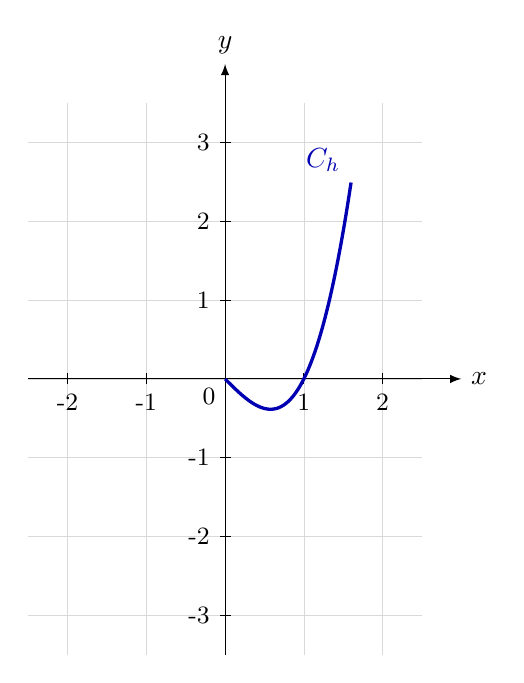
\begin{tikzpicture}[scale=1, >=latex]
    \draw[very thin, color=gray!30] (-2.5,-3.5) grid (2.5,3.5);
    \draw[->] (-2.5,0) -- (3,0) node[right] {$x$};
    \draw[->] (0,-3.5) -- (0,4) node[above] {$y$};
    
    \foreach \x in {-2,-1,1,2}
        \draw (\x,2pt) -- (\x,-2pt) node[below, font=\small] {\x};
    \foreach \y in {-3,-2,-1,1,2,3}
        \draw (2pt,\y) -- (-2pt,\y) node[left, font=\small] {\y};
    \node[below left, font=\small] at (0,0) {$0$};
    
    % h(x) = x^3 - x part (for x >= 0)
    \draw[very thick, color=blue!70!black, samples=100, smooth, domain=0:1.6] plot (\x, {\x*\x*\x - \x}) node[above left] {$C_h$};
\end{tikzpicture}
\end{center}

\begin{alist}
\item Να αποδείξετε ότι η συνάρτηση $h$ είναι περιττή.
\monades{03}

\item Να συμπληρώσετε το παραπάνω σχήμα ώστε να παριστάνει τη γραφική παράσταση της συνάρτησης $h$.
\monades{04}

\item Χωρίς να χρησιμοποιήσετε το παραπάνω σχήμα, να βρείτε τα σημεία τομής της γραφικής παράστασης της συνάρτησης $h$ με τον άξονα $x'x$.
\monades{08}

\item Αν $x \geq 0$ να αποδείξετε ότι: η γραφική παράσταση της συνάρτησης $g$ βρίσκεται πάνω από την ευθεία $\varepsilon: y = x$ αν και μόνο αν η γραφική παράσταση της $h$ βρίσκεται κάτω από τον άξονα $x'x$.
\monades{10}
\end{alist}
